
With this snapshot program, we propose to use HST's WFC3-IR detector
to discover the first multiply-imaged SN behind a strong lensing
galaxy cluster, setting the gold standard for future strong lensing
time delay measurements.  In recent years HST programs such as CLASH
and the Hubble Frontier Fields have built up a deep trove of WFC3-IR
imaging on strong-lensing galaxy clusters at redshifts $z\sim0.5$.
Many of these clusters have dozens of multiply-imaged background
galaxies at redshifts $1\lesssim z \lesssim 6$, which have been used
to produce well-constrained models of the cluster lensing potential.
When a SN inevitably appears within one of these multiply-imaged
galaxies, it will of course be multiply-imaged itself.  With that SN
we could measure a time delay distance with better than 6\%
precision, providing a unique and powerful
constraint on \Ho\ and dark energy.  With deep template imaging for
over 25 rich clusters in hand, {\bf \em we now have a viable pathway
to discover the first ever multiply-imaged SN with a small, single-cycle
snapshot program.}


\medskip
\noindent {\bf Time Delay Cosmography}

As light from a distant source passes through a galaxy cluster,
strong gravitational lensing causes multiple images to appear to the
observer, with a time separation between the images given by


\vspace{-5mm}
\begin{tabular}{p{5.5cm}r}
% \dt = \frac{\Dl \Ds}{\Dls} ( 1 + z_l ) \phi
{\begin{align}
%\begin{equation}\label{eq:dt}
 %  \dt = \frac{\Dl \Ds}{\Dls} ( 1 + z_l ) \phi
%\end{equation}
  \dt &= \frac{\Dl \Ds}{c\,\Dls} ( 1 + z_L ) \phi \label{eq:dt} \\
  \phi &= \frac{1}{2}(\theta-\beta)^2 - \psi(\theta) \label{eq:phi}
\end{align}}
&
\hspace{1cm}
\raisebox{-30mm}{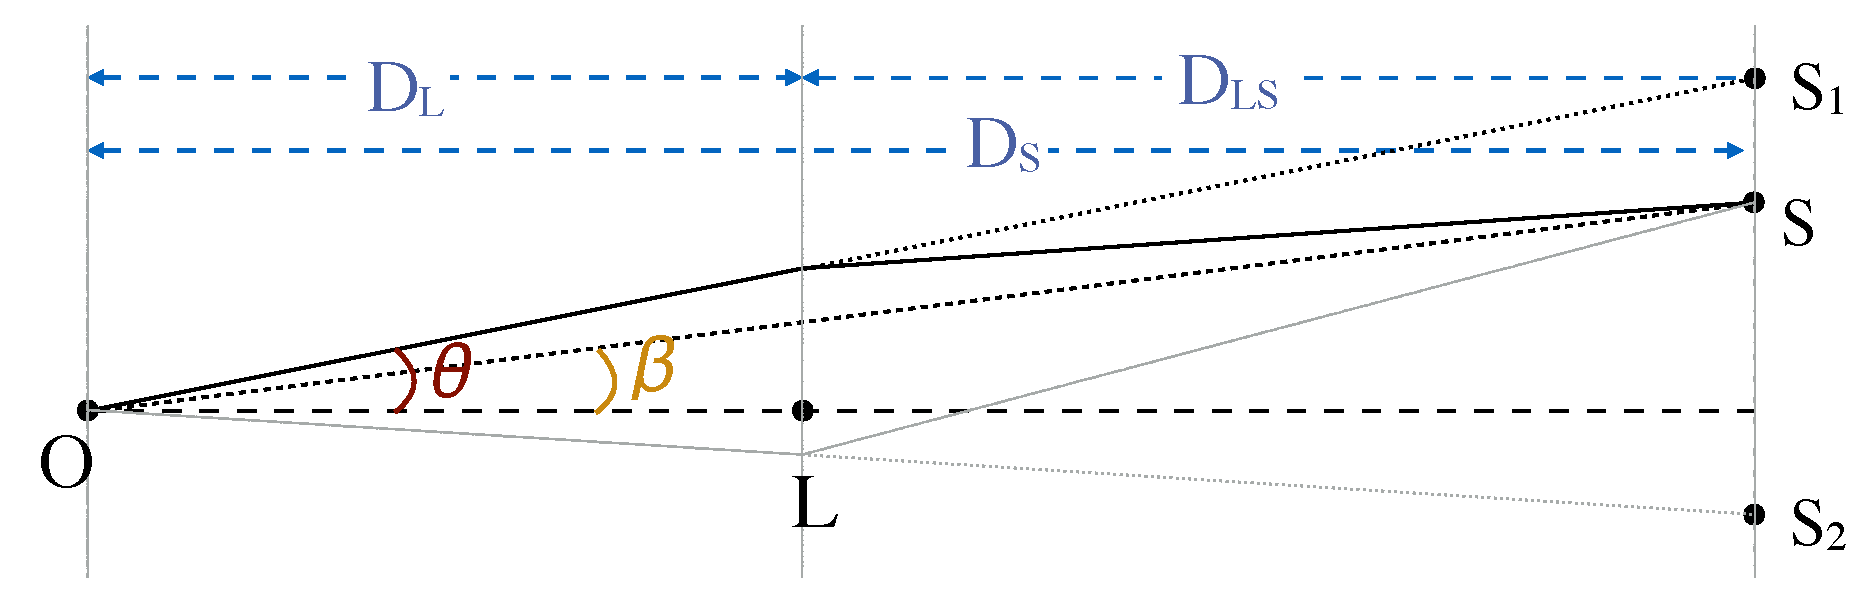
\includegraphics[width=0.5\textwidth]{FIG/lensingGeometry2}}
%\raisebox{-30mm}{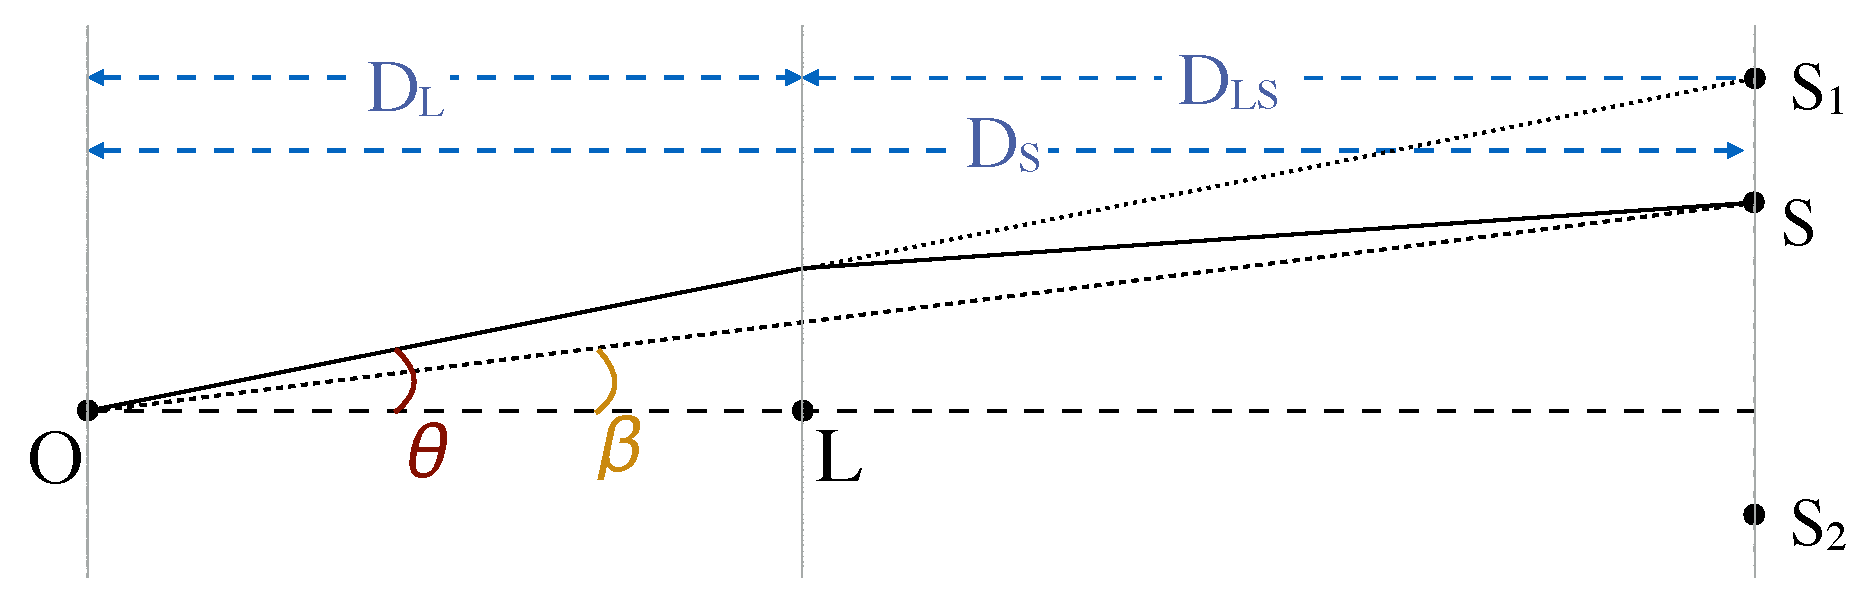
\includegraphics[width=0.5\textwidth]{FIG/lensingGeometry}}
\end{tabular}


\noindent where the redshift of the lens is $z_L$, while \Dl, \Ds, 
and \Dls\ are angular diamater distances from the observer to the
lens, observer to source, and lens to source, respectively.  The time
delay potential, $\phi$, is given in Eq.~\ref{eq:phi}. The first term
gives the geometric delay due to light rays following different path
lengths to the observer, and the second term, $\psi$, is the
relativistic component due to differing values of the gravitational
potential along each path.

Each of the distances in Equation~\ref{eq:dt} carries a factor
of \Ho$^{-1}$, so if the lensing potential $\phi$ is well known, then a
time delay measurement provides a direct measurement of the Hubble
constant.  The distance ratio $\Dl\Ds/\Dls$ also has
unusual sensitivities to cosmological parameters as a function of
redshift that make this technique a particularly useful probe of
dynamic dark energy models \citep{Linder:2011}.

\citet{Refsdal:1964} first proposed the use of SN time delays as 
a means to measure \Ho.  Now 50 years later, this has not yet been
achieved, primarily due to the small number of very well analyzed
gravitational lenses ($\sim$dozens), and the short visibility window
for any given high-$z$ SN event ($\sim$a few weeks).  Only recently
have we begun to realize the potential in this technique with the
recent measurement of a few dozen time delays of quasars, being lensed
typically by a single foreground galaxy \citep{Jackson:2007}. Among
these, only a handful have time delays measured with particularly high
precision \citep[e.g.]{Suyu:2010,Suyu:2013}.  These quasar lenses
generally suffer from a number of serious concerns, notably: (1) the
lensing potential is poorly constrained due to inherent degeneracies
and insufficient constraints; (2) the time delays and angular
separations are quite small (tens of days, fractions of an arcsecond);
and (3) the source is continuously variable, requiring many years of
stable monitoring to resolve phase degeneracies.  Wide-field surveys
in the coming decade could deliver $>$100 quasar time delays, but
these problems represent unavoidable systematic biases for this
sample.


\medskip
\noindent {\bf The SN Time Delay Advantage}
 
In Cycle 22, HST has just achieved a new capability for the discovery
of a strongly-lensed SN. The first key advancement was the
availability of WFC3-IR, which allows HST imaging surveys to capture
high-$z$ SN at the peak of their SED profile in rest-frame optical
bands \citep{Rodney:2012,Jones:2013}.  Ground-based surveys and even
HST/ACS programs have searched for multiply-imaged SN in the past, but
none have had the capability to detect even highly magnified SN at
$z>2$ \citep[e.g.][]{Dawson:2009,Sand:2011}.  With WFC3-IR, \Hubble\
now has access to a much larger survey volume with each pointing.

A WFC3-IR program targeting massive clusters, such as CLASH or the
Hubble Frontier Fields, could in principal have caught a strongly
lensed SN already, but in practice the likelihood of such a find was
vanishingly small.  The CLASH team collected WFC3-IR imaging of 25
clusters over 3-years, but the time separation between the first and
last image on any single cluster was never more than a few months.
However, these programs -- along with other WFC3-IR cluster imaging
campaigns -- have now provided the second critical advance: deep IR
template imaging of massive clusters from which to construct
difference images for SN discovery.  These HST programs have also led
to an explosion of detailed mass modeling for strong-lensing clusters,
providing well-defined lensing potentials that will be crucial for
evaluating a multiply-imaged SN when one is found.  

Our snapshot program will capitalize on this rich new treasury of IR
cluster imaging in the HST archive, opening the door for a pioneering
time delay distance measurement with the discovery of one or more
strongly lensed SN behind a galaxy cluster.  We will target
well-studied massive clusters that act as especially strong lenses
(Table~\ref{tab:clusters}). For each of these clusters we have dozens
of known multiply-imaged galaxies, and we already have
state-of-the-art lens models in
hand \citep[e.g.][]{Zitrin:2011a,Zitrin:2011b,Zitrin:2012a,Zitrin:2012b,Zitrin:2013}.
Wherever a multiply-imaged SN should appear, {\bf \em we will be
starting out with much better constraints on the lensing potential
$\phi$} than are available for existing quasar time-delay lenses. In
addition to improving the quality of the time-delay cosmography, this
fore-knowledge of the lensing potential will also be crucial for
quickly evaluating any lensed SN candidates we discover, to weed out
impostors before investing precious follow-up time.

Furthermore, {\bf \em the SN we discover behind these clusters will be
inherently better time-delay sources} than the existing sample of
quasars.  Typical time delays through our target clusters are months
or years (not days or weeks as for many lensed quasars), allowing for
more precise measurements of \dt, with ample time to prepare for the
appearance of the second image.  Also, the SN light curve has a single
peak, so there is no possibility of phase ambiguity, and the age of a
SN relative to explosion can be precisely defined from light curve
shape and color, or from spectroscopic
cross-correlation \citep{Filippenko:1997,Blondin:2007}.  Thus the time
delay measurement does not require continuous long-term monitoring,
and can be made with minimal systematic uncertainties.

% Finally, if the SN is of Type Ia (a likely prospect), then light curve
% fitting can provide a luminosity distance measurement with $\sim$8\%
% precision \citep{Phillips:1993}.  Galaxy cluster distances can also be
% estimated using the Sunyaev-Zeldovich effect and x-ray cluster
% luminosities \citep{Silk:1978}.  This means that in addition to the
% time delay distance ratio (\Dl\Ds/\Dls) we can also measure
% independent distances to both the lens and the source.  A \SNIa\ that
% is multiply-imaged by a galaxy cluster would therefore provide a
% unique chance to test for systematic biases in these distance
% estimators.
% %, or even to perform the distance-duality test: if the
% %ratio $\eta_{DD} = D_{S}^{(L)} / ( D_{S}^{(A)}(1+z_S)^2 )$ deviates
% %from unity, then this would signal systematic errors in one or more
% %distances, or a fundamental flaw in the concordance cosmology.


% The large angular separations between our lensed sources and their
% unlensed sight-lines will allow for very precise astrometry that is
% free of systematics due to source blending.  



\medskip
\noindent {\bf The HST Snapshot Search Strategy }

Since Cycle 17, HST surveys of strong lensing clusters (notably CLASH
and the Frontier Fields) have been investing hundreds of orbits in deep
WFC3-IR imaging.  With these templates in hand, the most efficient
way to discover high-$z$ strongly lensed SN is through a relatively
small snapshot program.    To estimate the number of snapshots we
need, we use a tabulation of the number of known multiply-imaged
galaxies in the fields of our target clusters
(Table~\ref{tab:clusters}).  This is a conservative approach, as it is
quite possible to detect a multiply-imaged SN even if the host galaxy
is well below the current detection thresholds for these cluster
fields. The total yield of strongly-lensed SN per snapshot is then

\begin{equation} \label{eq:Nsn}
N_{SN} = SNR_{M} \times M_{gal} \times N_{gal} \times t_{vis},
\end{equation}

\noindent where $SNR_{M^*}$ is the SN rate per unit mass, $M_{gal}$ is
the average mass of a multiply-imaged galaxy, $N_{gal}$ is the number
of multiply imaged galaxies in the field, and $t_{vis}$ is the length
of time that any given SN is visible to our snapshot survey.  Most of
the lensed systems in our target list are at $z\sim 2$, in an era near
the peak of the cosmic star formation history. This should substantially
enhance the rate of both Type Ia and Type II SN, but we conservatively
assume that our average lensed galaxy is generating SN at a rate
similar to an Sb galaxy in our local universe: $SNR_{M} \sim 0.1$ for
both \SNIa\ and SN II \citep{Mannucci:2005}.  We adopt an average
stellar mass of $M_{gal}=10^{10.7} \Msun$ \citep{Tomczak:2013}, and
use the census of multiply-imaged systems in Table~\ref{tab:clusters}
to predict an average of $N_{gal}\sim 35$ lensed galaxy images per
cluster.\footnote{Note that we count each separate image of a
multiple-image set except the last one (typically the most highly
magnified).  The time delay between each image is of order months or
years, so each snapshot is essentially observing the same galaxy at
multiple widely-spaced epochs that can be treated as independent for
the purpose of SN discovery. The last image is not counted because we
can not measure a time delay from the last appearance of a
multiply-imaged SN.}

%\begin{wrapfigure}{r}{0.3\textwidth}
%\minipage[r]{0.29\textwidth}
   
\begin{wraptable}{r}{2.25in}
 \caption{Detection Limits \label{tab:detectionLimits}}
 \begin{tabular}{ccc}
  \toprule
  \toprule
   WFC3/IR & Exp.Time & m$_{lim}$ $^{*}$ \\
   Filter  &  [min] &  [AB mag] \\
   \midrule
   F110W   &    12  &   26.3 \\
   F110W   &    20  &   26.6 \\
   F110W   &    30  &   26.9 \\
   F140W   &    12  &   25.9 \\
   F140W   &    20  &   26.2 \\ 
   F140W   &    30  &   26.5 \\
  \bottomrule
 \multicolumn{3}{p{2.6in}}{$^*$\,Apparent magnitude that yields S/N of 5 (optimum S/N$\sim$10) in the given exposure time.}
\end{tabular}
\end{wraptable}




%\end{minipage}
%\end{wrapfigure}

To maximize the flexibility for scheduling, we consider snapshots with
12, 20 and 30 minutes of exposure time ($\sim$22, 30, and 40 min with
overhead).  These snapshots reach a depth of 25-26 AB mag in the F110W
and F140W filters (Table~\ref{tab:detectionLimits}).  To describe a
realistic distribution of SN visibility times, $t_{vis}$, we use a
census of magnifications and redshifts from all multiply-imaged
galaxies in three of our primary cluster targets
(Figure~\ref{fig:tvis}).  We then use simulated SN light curves to
measure the length of time each SN stays above our detection
threshold, finding an average $t_{vis}\sim 30$ days for \SNIa\ and
$\sim$20 days for SN II.

Inserting these estimates into Eq.~\ref{eq:Nsn}, we find $N_{SN}\sim
0.02$ SN per snapshot, including both Type Ia and II.  To give this
program a realistic chance at discovering a strongly lensed SN in
Cycle 22, we request 200 snapshots, which would yield a sample of
$\sim 4 ^{+3}_{-2}$ SN in one year if all snaps were executed.  With a
realistic snapshot execution rate of $\sim$30\%, that sample drops to
$\sim$one.  These are perilously small sample sizes, but given the
conservative estimates used in this prediction, we expect that a
200-snap allocation will be sufficient to deliver at least one
strongly lensed SN in Cycle 22.  Even just a single detection will
nevertheless be an extraordinary step forward for time delay
cosmography. 

Finally, we note that this snapshot program is designed only for
discovery. Follow-up observations will come from accompanying GO
program, using 12 orbits with ToO observations for immediate
confirmation of a SN candidate and measurement of the light curve.
Sometime in the future, a return campaign to catch the next image
would be needed to complete the time delay measurement, using HST,
ground-based AO systems, or possibly JWST, depending on the length of
the delay.


\medskip
\noindent{\bf Lensed \SNIa\ Probing Cluster Models} 
We could find lensed SN Ia with significant magnification that do not
have multiple images, adding to the sample of SN lensing probes
(Patel+ 2014, Nordin+ 2014).  Classification and light curve
measurement could be done with FrontierSN follow-up orbits


\begin{table}
\caption{Cluster Target List\label{tab:clusters}}
\begin{tabu}{llllcl}
\toprule
\toprule
Cluster & R.A. & Decl. & z & N$_{im}$ $^*$ & References \\
\midrule
\rowfont{\color{blue}}
Abell 2744\dag & 00:14:23.4 & -30:23:26 & 0.31 & 43  & Merten et al. 2011                                         \\
CL0024         & 00:26:35.0 & +17:09:43 & 0.39 & 20  & Zitrin et al. 2009a                                        \\
El Gordo       & 01:02:52.5 & -49:14:58 & 0.87 & 11  & Zitrin et al. 2013b                                        \\
\rowfont{\color{blue}}
Abell 370\dag  & 02:39:52.8 & -01:34:36 & 0.37 & 36  & Richard et al. 2009, ZFF                                   \\
Abell 383      & 02:48:03.4 & -03:31:44 & 0.19 & 18  & Zitrin et al. 2011b                                        \\
\rowfont{\color{blue}}
MACS0416\dag   & 04:16:08.4 & -24:04:21 & 0.40 & 36  & Zitrin et al. 2013                                         \\
MACS0647       & 06:47:50.3 & +70:14:55 & 0.58 & 20  & Zitrin et al. 2011, Coe et al. 2013                        \\
Bullet-a       & 06:58:37.9 & -55:57:00 & 0.3  & 10  & Bradac et al. **                                           \\
Bullet-b       & 06:58:37.9 & -55:57:00 & 0.3  & 11  & Bradac et al. **                                           \\
MACS0717-a     & 07:17:35.6 & +37:44:44 & 0.55 & 18  & Zitrin et al. 2009b, Limousin et al. 2012, Z14             \\
MACS0717-b     & 07:17:35.6 & +37:44:44 & 0.55 & 18  & Zitrin et al. 2009b, Limousin et al. 2012, Z14             \\
MACS0744       & 07:44:52.8 & +39:27:24 & 0.70 & 14  & Zitrin et al. 2011; 2014 in prep                           \\
Abell 611      & 08:00:56.8 & +36:03:23 & 0.21 & 12  & Newman et al. 2013, Z14                                    \\
\rowfont{\color{blue}}
MACS1149\dag   & 11:49:35.7 & +22:23:55 & 0.54 & 29  & Zitrin  \&  Broadhurst 2009, Zheng et al. 2012             \\
\rowfont{\color{blue}}
MACS1206\dag   & 12:06:12.1 & -08:48:04 & 0.44 & 33  & Ebeling et al. 2009, Zitrin et al. 2012                    \\
\rowfont{\color{blue}}
Abell 1689\dag & 13:11:34.2 & -01:21:56 & 0.19 & 117 & Broadhurst et al. 2005, Coe et al. 2010, Diego et al. 2014 \\
\rowfont{\color{blue}}
Abell 1703\dag & 13:15:03.7 & +51:49:27 & 0.28 & 36  & Limousin et al. 200*, Zitrin et al. 2010                   \\
RXJ1347        & 13:47:31.1 & -11:45:12 & 0.45 & 14  & K\"ohlinger \&  Schmidt 2014                               \\
MS1358         & 13:59:48.7 & +62:30:48 & 0.33 & 13  & Zitrin et al. 2011c                                        \\
Abell 1835     & 14:01:02.0 & +02:52:45 & 0.25 & 17  & Richard et al. 2010, Morandi et al. 2012                   \\
Abell 2218     & 16:35:54.0 & +66:13:00 & 0.18 & 18  & Kneib et al. 2004                                          \\
Abell 2261     & 17:22:27.2 & +32:07:57 & 0.22 & 18  & Coe et al. 2012                                            \\
MACS1931       & 19:31:49.6 & -26:34:32 & 0.35 & 10  & Z14                                                        \\
MACS2129       & 21:29:26.1 & -07:41:28 & 0.57 & 14  & Zitrin et al. 2011; Z14                                    \\
\rowfont{\color{blue}}
RXJ2248\dag    & 22:48:44.0 & -44:31:51 & 0.35 & 28  & Monna et al. 2013                                          \\
\bottomrule
% MACS0329   & 03:29:41.6 & -02:11:46 & 0.45 & 11 & Zitrin et al. 2012, Z14                       \\
% MACS0451   & 04:51:54.6 & +00:06:17 & 0.43 & 11                                                 \\
% MACS0454   & 04:54:11.1 & -03:00:53 & 0.54 & 11 & Zitrin et al. 2011                            \\
% CL1226     & 12:26:58.2 & +33:32:48 & 0.89 & 11 & Z14                                           \\
% MACS1423   & 14:23:48.3 & +24:04:47 & 0.54 & 11 & Limousin et al. 2010, Zitrin et al. 2011, Z14 \\
% MACS1720   & 17:20:16.8 & +35:36:26 & 0.39 & 11 & Z14                                           \\
% Abell 2390 & 21:53:55.8 & +17:43:34 & 0.23 & 7  & Frye et al. 1998                              \\
% MS2137     & 21:40:15.2 & -23:39:40 & 0.31 & 7  & Newman et al. 2013, Z14                       \\
% RXJ2129    & 21:29:40.0 & +00:05:21 & 0.23 & 9  & Richard et al. 2010, Z14                      \\
%\enddata
 \multicolumn{6}{p{\textwidth}}{* Approximate number of known strongly-lensed galaxy images
   within the WFC3-IR FOV, counting all instances of each lensed galaxy
   except the last (i.e. all independent lensed galaxy images that
   could deliver a SN time delay measurement).}\\
 \multicolumn{6}{p{\textwidth}}{ \textcolor{blue}{$\dagger$ Primary targets.} We will allocate more
   snapshots to these clusters that have especially strong lenses with
   many multiply-imaged galaxies and particularly good lens models.
   The unweighted average $N_{im}$ is $\sim$25, but we expect this
   weighted snapshot allocation to result in an actual mean of
   $N_{im}\sim 35$.}\\
%\tablenotetext{**}{ Key or latest references for the multiple image
%  compilation in each cluster. Z14 stands for ``Zitrin et al. 2014 in
%  prep" is a soon to be public paper describing our high-end mass
%  models already available online for the community, and multiple
%  images, for all 25 CLASH clusters. ``ZFF" refers to the internal
%  list of the Frontier Fields map making groups, for which Co-PI
%  Zitrin has contributed significantly for revising the multiple
%  images.}
\end{tabu}
\end{table}



\insertfig{FIG/lightcurves.pdf}{ \label{fig:lightcurves} Lensed SN
    light curves }

\insertfig{FIG/tvis_muz_30min.pdf}{\label{fig:tvis} Visibility time
for lensed SN. }




